\documentclass[aspectratio=169,11pt]{beamer}
\usetheme{Madrid}
\usecolortheme{seahorse}
\setbeamertemplate{navigation symbols}{}
\setbeamertemplate{footline}[frame number]
\usepackage{graphicx}
\usepackage{amsmath,amssymb}
\usepackage{booktabs}

\definecolor{teal}{HTML}{167568}
\definecolor{sblue}{HTML}{376687}
\definecolor{amber}{HTML}{C2821E}
\setbeamercolor{title}{fg=sblue}
\setbeamercolor{frametitle}{fg=sblue}
\setbeamercolor{structure}{fg=sblue}
\setbeamercolor{alerted text}{fg=teal}

\title[3D Gaussian Splat SLAM]{Splatt3R-SLAM:\\From Image Pairs to Persistent Maps}
\subtitle{Real-time photorealistic dense SLAM with 3D Gaussian primitives}
\author{Zelong Li}
\institute{MSc Computer Science --- University of Amsterdam\\[2pt]\small Supervisors: Prof. Martin Oswald \quad Dr. Qi Zhang}
\date{October 2026}

\newcommand{\gauss}[3]{\ensuremath{#1,\!#2,\!#3}}

\begin{document}

% 1 ----------------------------------------------------------------------
\begin{frame}[plain]
  \titlepage
\end{frame}

% 2 ----------------------------------------------------------------------
\begin{frame}{Talk outline}
  \vspace{4pt}
  \begin{columns}
    \column{.5\textwidth}
    \begin{enumerate}
      \item The problem: an image pair is not a map
      \item The idea: share the anchor
      \item The method: predict -- anchor -- refine
    \end{enumerate}
    \column{.5\textwidth}
    \begin{enumerate}\setcounter{enumi}{3}
      \item Results on real sequences
      \item Limitations and conclusion
    \end{enumerate}
  \end{columns}
  \vspace{6pt}
  {\centering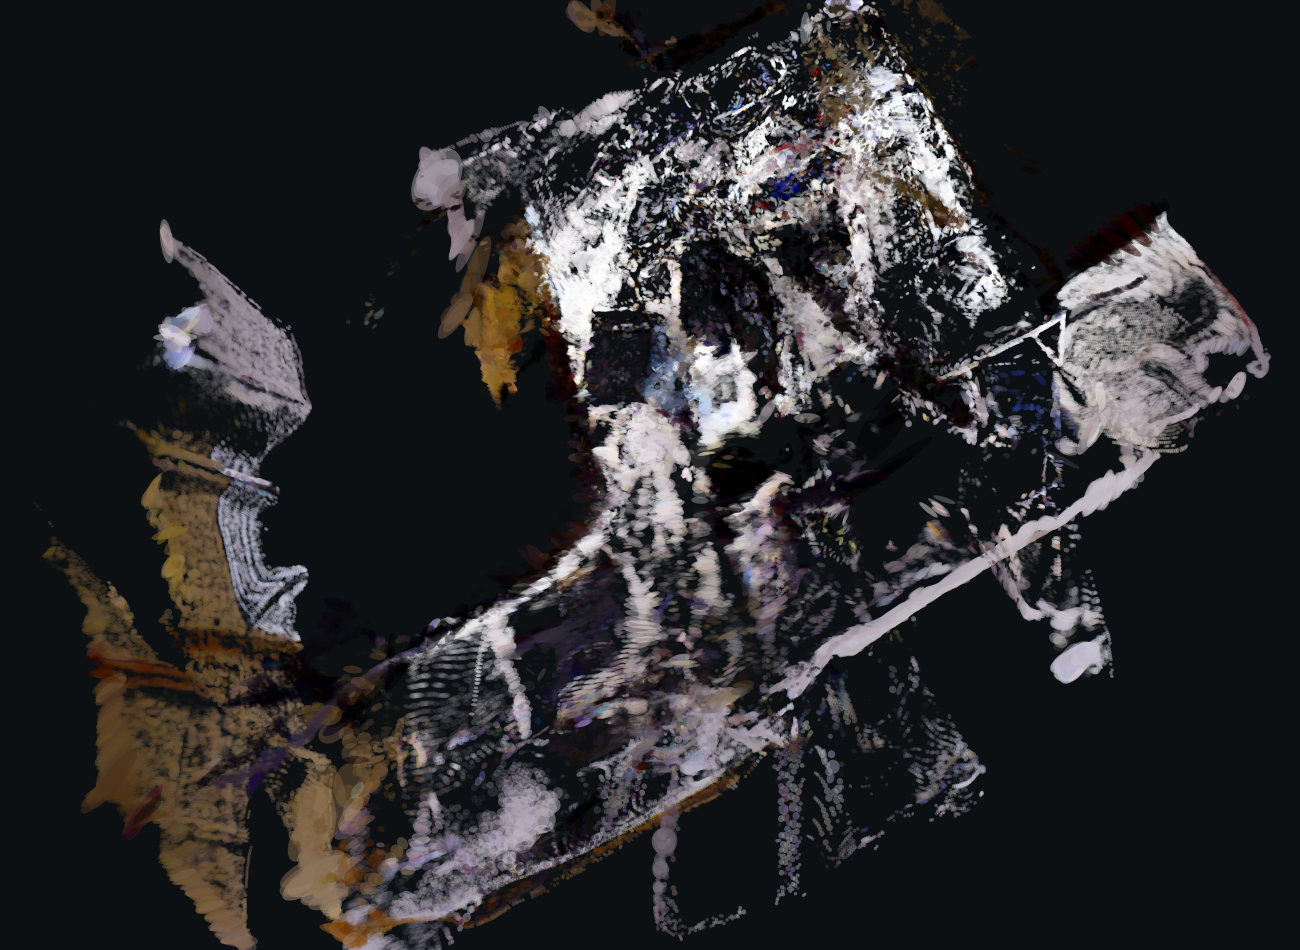
\includegraphics[height=3.4cm]{assets/gauss_desk.png}\par}
  {\footnotesize\centering The map as individual Gaussian primitives\par}
\end{frame}

% 3 ----------------------------------------------------------------------
\begin{frame}{An image pair is not a map}
  \begin{columns}
    \column{.42\textwidth}
    \alert{One pair gives a useful local result.}\\[4pt]
    But a video sequence adds problems a two-view model never sees:
    \begin{itemize}\small
      \item every pair lives in its own camera frame;
      \item many keyframes place colour on one ray;
      \item a loop closure changes where old content belongs.
    \end{itemize}
    \column{.58\textwidth}
    \centering
    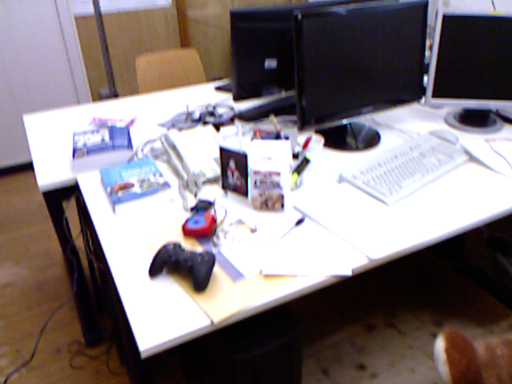
\includegraphics[width=.46\textwidth]{assets/desk_gt.png}\hfill
    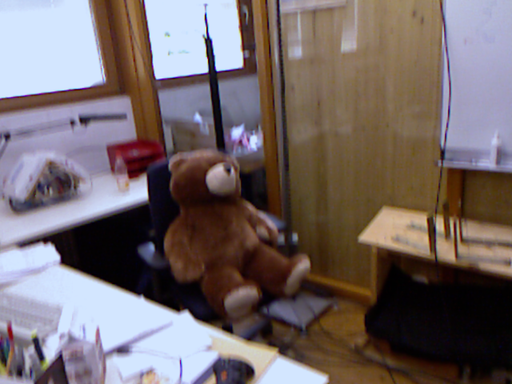
\includegraphics[width=.46\textwidth]{assets/tum360_gt.png}\\[4pt]
    {\footnotesize Two real input views (TUM)}
  \end{columns}
\end{frame}

% 4 ----------------------------------------------------------------------
\begin{frame}{What a persistent map must survive}
  \vspace{2pt}
  \begin{columns}[t]
    \column{.31\textwidth}
    \centering\color{sblue}\large\textbf{Revit}\\[3pt]
    \color{black}\small A later camera must still localise.
    \column{.31\textwidth}
    \centering\color{amber}\large\textbf{Correct}\\[3pt]
    \color{black}\small Loop closure must move old content.
    \column{.31\textwidth}
    \centering\color{teal}\large\textbf{Render}\\[3pt]
    \color{black}\small A new view must look like the scene.
  \end{columns}
  \vspace{10pt}
  \begin{block}{Central requirement}
    Tracking, pose correction, and rendering must describe the \textbf{same} scene.
  \end{block}
\end{frame}

% 5 ----------------------------------------------------------------------
\begin{frame}{The thesis: share the anchor}
  \large
  Store the local Gaussian map \textbf{and} the cameras that supervise it under the \alert{same keyframe anchor}.
  \normalsize
  \vspace{8pt}
  \begin{equation*}
    T_{WC_f}^{-1}\,T_{WC_k} = T_{C_k C_f}^{-1}
  \end{equation*}
  \vspace{2pt}
  \begin{itemize}
    \item a pose correction updates one anchor transform;
    \item the linked map and every observation camera move together;
    \item their relative relation is preserved exactly.
  \end{itemize}
\end{frame}

% 6 ----------------------------------------------------------------------
\begin{frame}{Method: one shared predictor, two lanes}
  \small
  \begin{columns}
    \column{.5\textwidth}
    \textbf{Geometry lane}\\[2pt]
    pointmaps and matching features feed the tracker and pose graph.
    \vspace{8pt}\\
    \textbf{Gaussian lane}\\[2pt]
    one primitive per valid pixel:
    \[
      \Sigma_n = R(q_n)\,\mathrm{diag}(s_n^2)\,R(q_n)^\top
    \]
    \column{.5\textwidth}
    \centering
    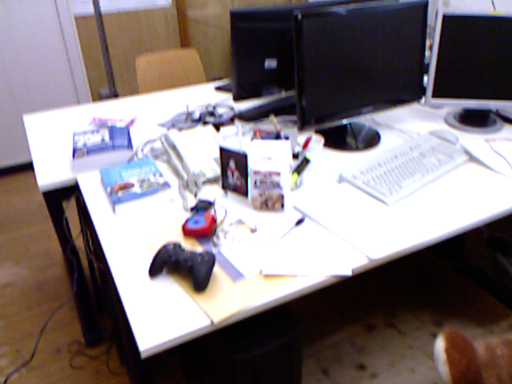
\includegraphics[width=.44\textwidth]{assets/desk_gt.png}\hfill
    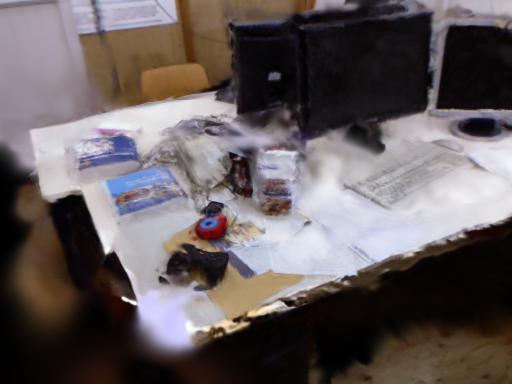
\includegraphics[width=.44\textwidth]{assets/desk_ours.png}\\[4pt]
    {\footnotesize Real view (left) and predicted map}
  \end{columns}
\end{frame}

% 7 ----------------------------------------------------------------------
\begin{frame}{Refine: use the sequence without moving the tracker}
  \begin{columns}
    \column{.56\textwidth}
    A separate process repeatedly:
    \begin{enumerate}\small
      \item samples a tracked view (reservoir + recent ring);
      \item renders the assembled Gaussian map;
      \item measures $0.8\,L_1 + 0.2\,\text{D-SSIM}$;
      \item takes an Adam step on appearance only.
    \end{enumerate}
    \vspace{4pt}
    \alert{Gradients never update poses or tracking weights.}
    \column{.44\textwidth}
    \centering
    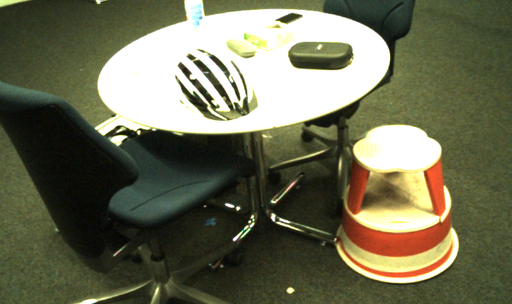
\includegraphics[width=.95\textwidth]{assets/eth_table_gt.png}\\[3pt]
    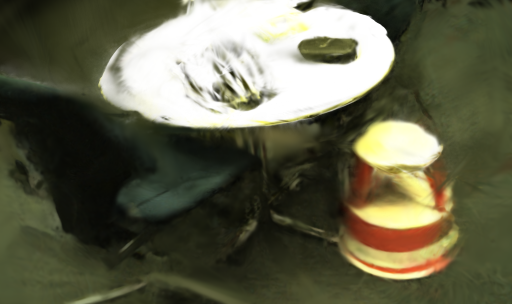
\includegraphics[width=.95\textwidth]{assets/eth_table.png}\\[3pt]
    {\footnotesize ETH3D: ground truth (top), ours (bottom)}
  \end{columns}
\end{frame}

% 8 ----------------------------------------------------------------------
\begin{frame}{System: concurrent processes}
  \small
  \begin{center}
  \begin{tabular}{@{}lll@{}}
    \toprule
    Device & Components & Role\\
    \midrule
    GPU 0 & Tracker, Backend, Visualiser & predict, track, pose graph, render \\
    CPU  & Supervision frames, Snapshot & sampling pool, versioned map \\
    GPU 1 & Refiner & appearance optimisation \\
    \bottomrule
  \end{tabular}
  \end{center}
  \vspace{2pt}
  \begin{itemize}
    \item SharedKeyframes exchanged through CUDA IPC;
    \item supervision and snapshots through CPU shared memory;
    \item tracking owns poses; refinement only publishes maps.
  \end{itemize}
\end{frame}

% 9 ----------------------------------------------------------------------
\begin{frame}{Results: real sequences}
  \begin{columns}
    \column{.5\textwidth}
    \centering
    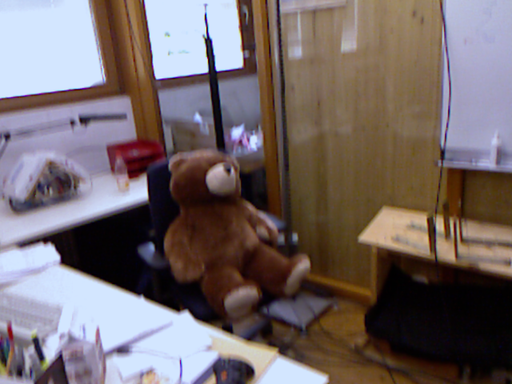
\includegraphics[width=.95\textwidth]{assets/tum360_gt.png}\\[3pt]
    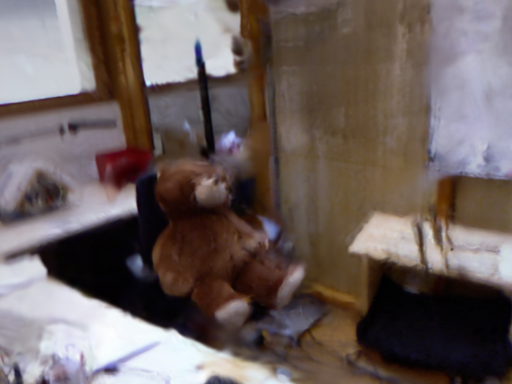
\includegraphics[width=.95\textwidth]{assets/tum360_ours.png}\\[3pt]
    {\footnotesize TUM fr1/360: ground truth (top), ours (bottom)}
    \column{.5\textwidth}
    \centering
    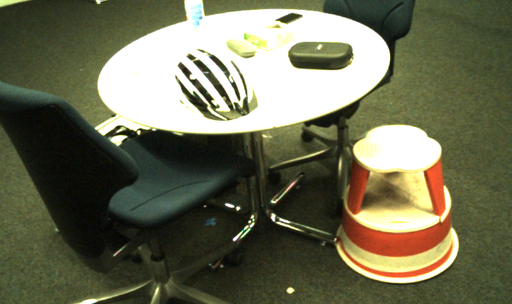
\includegraphics[width=.95\textwidth]{assets/eth_table_gt.png}\\[3pt]
    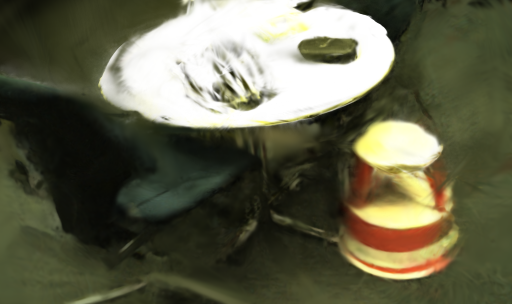
\includegraphics[width=.95\textwidth]{assets/eth_table.png}\\[3pt]
    {\footnotesize ETH3D table: ground truth (top), ours (bottom)}
  \end{columns}
\end{frame}

% 10 ---------------------------------------------------------------------
\begin{frame}{Quantitative comparison (common renderer)}
  \small
  \begin{center}
  \begin{tabular}{@{}lccc@{}}
    \toprule
    Scene (real) & Photo-SLAM & MonoGS & \textbf{Ours}\\
    \midrule
    TUM desk PSNR (dB)        & 10.67 & 13.91 & \textbf{13.95}\\
    TUM desk LPIPS (Alex)$\downarrow$ & 0.46 & \textbf{0.395} & 0.411\\
    \bottomrule
  \end{tabular}
  \end{center}
  \vspace{4pt}
  \begin{itemize}\small
    \item real desk: \alert{$+3.28$\,dB over Photo-SLAM};
    \item parity with MonoGS, with slightly higher LPIPS;
    \item on the synthetic Replica benchmark: $23.02$\,dB, 8/8 scene wins.
  \end{itemize}
\end{frame}

% 11 ---------------------------------------------------------------------
\begin{frame}{Limitations}
  \begin{itemize}
    \item tracking is inherited from MASt3R-SLAM, not a new contribution;
    \item full maps are large ($\sim$2.4\,M primitives) --- not yet compact;
    \item thin structures and cables carry the most residual blur;
    \item single runs can hide system variance;
    \item real-world novel-view benchmarks remain sparse in the literature.
  \end{itemize}
\end{frame}

% 12 ---------------------------------------------------------------------
\begin{frame}{Conclusion}
  \large
  \begin{itemize}
    \item[\color{teal}$\blacktriangleright$] \textbf{Predict}: dense local Gaussians in one pass;
    \item[\color{amber}$\blacktriangleright$] \textbf{Anchor}: corrections move map and cameras together;
    \item[\color{sblue}$\blacktriangleright$] \textbf{Refine}: sequence RGB improves appearance downstream.
  \end{itemize}
  \normalsize
  \vspace{6pt}
  \begin{block}{One idea}
    Give the local map and its observation cameras the same keyframe anchor.
  \end{block}
\end{frame}

% 13 backup --------------------------------------------------------------
\appendix
\begin{frame}{Backup: related-work positioning}
  \small
  \begin{center}
  \begin{tabular}{@{}ll@{}}
    \toprule
    System & Positioning\\
    \midrule
    Photo-SLAM, MonoGS & optimisation-first Gaussian SLAM (CVPR'24)\\
    Splat-SLAM, SplaTAM & global / RGB-D Gaussian maps (2024)\\
    SEGS-SLAM & structure-enhanced, appearance embedding (2025)\\
    \textbf{Splatt3R-SLAM} & prediction-first priors + shared anchors\\
    \bottomrule
  \end{tabular}
  \end{center}
\end{frame}

\begin{frame}{Backup: primary settings}
  \small
  \begin{tabular}{@{}ll@{}}
    \toprule
    Field & Value\\
    \midrule
    Input & monocular RGB\\
    Predictor & frozen Splatt3R\\
    Refinement loss & $0.8\,L_1 + 0.2\,$D-SSIM\\
    Optimiser & Adam, appearance only\\
    Evaluation & common non-keyframes, GT Sim(3) alignment, full exported SH\\
    Metrics & PSNR, LPIPS-AlexNet\\
    \bottomrule
  \end{tabular}
\end{frame}

\end{document}
